\chapter{Comunicaciones Digitales Avanzadas}

\section*{El Teorema de Shannon}

\section{Modulación QPSK}
[falta explicar]

\section{Modulación MPSK}
[falta explicar]

\section{Modulación MQAM}
[falta explicar]


\section{Modulación basadas en constelaciones en gnuradio}

\subsection{Modulacion M-PAM}

En GNU Radio la modulación M-PAM se usa de manera indirecta, ya que el bloque que vamos a usar para la realizar la modulación digital pasobandas de orden M exige que la señal de entrada esté previamente modulada en M-PAM. \\

\begin{table}[h!]
	\captionsetup{justification = raggedright,singlelinecheck = false}
	\caption{\label{tabla:tabla9} Tabla de Verdad de la Modulación M-PAM}
	\begin{center}
		\scalebox{0.75}{
			\begin{tabular}{|l|l|l|}
				\hline
				\multicolumn{2}{|c|}{\textbf{Tabla de Verdad de la Modulación BPSK}}\\ \hline
				Clave & Fase  \\ \hline
				000	& 		 0 \\ \hline
				001	& 1 \\ \hline
				010	& 2 \\ \hline
				011	& 3 \\ \hline
				100	& 4 \\ \hline
				101	& 5 \\ \hline
				110	& 6 \\ \hline
				111	& 7 \\ \hline
		\end{tabular}}
	\end{center}
\end{table}

M-PAM se refiere a la modulación de la amplitud de los pulsos en M posibles valores. A diferencia de la modulación PAM (Pulse Amplitude Modulation), donde la amplitud de los pulsos es modulados por un mensaje analógico, en la modulación M-PAM el mensaje es una señal binaria. M-PAM no es una modulación usada de manera directa en GNU Radio, es más bien usada en sistemas que no requieren una portadora de radio como en algunos casos de comunicación por cable o por fibra óptica. 
La modulación M-PAM está dada por una tabla de verdad, donde cada símbolo (combinación de bits) se representa mediante un valor de amplitud, como en la tabla \ref{tabla:tabla10}. \\

%%%%%%%%%%%%%%%%%%%%%%%%%%%%%%%%%%%%%%%%%%%%%

\section{Curvas de BER}
En una comunicación Digital, BER (Bit Error Ratio) es el número de bits en un volumen de datos transmitidos que llegan alterados al receptor debido a su paso por el canal, donde la señal es afectada por el ruido, las interferencias o distorsiones. BER es el número de bits con errores dividido entre el total de bits transmitidos en un intervalo de estudio. Es usualmente medido en forma de porcentaje. La probabilidad de error $P_e$ es el valor esperado de la BER.  La BER puede ser considerada como una estimación aproximada de la probabilidad de pérdida de bits. \\

Ejemplo, supongamos que la secuencia transmitida es la siguiente: \\

0110001011 \\

pero que al receptor llegó lo siguiente: \\

0010101001 \\

El número de bits con errores son en este caso 3. La BER son 3 bits incorrectos divididos entre 10 bits transmitidos, lo cual resulta en una BER de 0.3 o 30$\%$.
La BER puede ser evaluada usando simulación estocástica computarizada, lo cual se conoce mejor como el método de Monte Carlo. Pero es bastante común su cálculo analítico asumiendo un sencillo modelo del canal de transmisión y una fuente de datos, en este caso uno de los modelos es el de Bernoulli. \\

%\vspace{250px}
\section{Curvas de BER comparativas de algunos de sistemas que funcionan con algunos métodos de modulación} 

%\setcounter{figure}{127}
\begin{figure}[h!]
	\captionsetup{justification = raggedright, singlelinecheck = false}
	\caption{Curvas de BER BPSK, QPSK, PSK} 
	\centering
	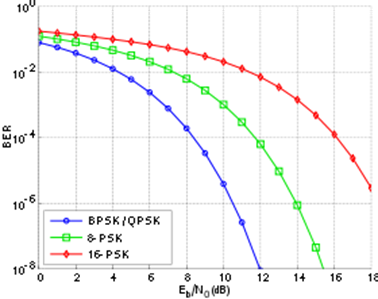
\includegraphics[scale=1]{Imagenes/Eb.png}
	\label{fig:Eb}
	%	\captionsetup{justification=raggedright,font={scriptsize,bf,it}}
	%	\caption*{fuente: \textcolor{
	%			Orange}{Tomada de Wikipedia}}
\end{figure}	


\vspace{200px}
\begin{figure}[h!]
	\captionsetup{justification = raggedright, singlelinecheck = false}
	\caption{Curva de BER BPSK con y sin Codificación Diferencial} 
	\centering
	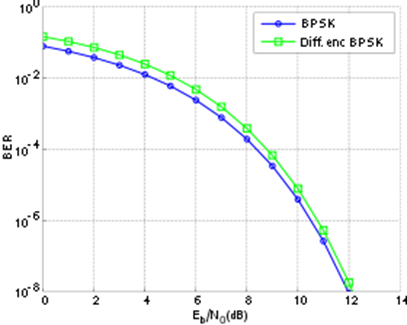
\includegraphics[scale=1]{Imagenes/Ber.png}
	\label{fig:Ber}
	%	\captionsetup{justification=raggedright,font={scriptsize,bf,it}}
	%	\caption*{fuente: \textcolor{
	%			Orange}{Tomada de Wikipedia}}
\end{figure}	

% \vspace{100px}
Las curvas de BER también pueden ser dadas en función de Es/No como se muestra en la siguiente figura.

\begin{figure}[h!]
	\captionsetup{justification = raggedright, singlelinecheck = false}
	\caption{Curvas de BER Diversas Modulaciones} 
	\centering
	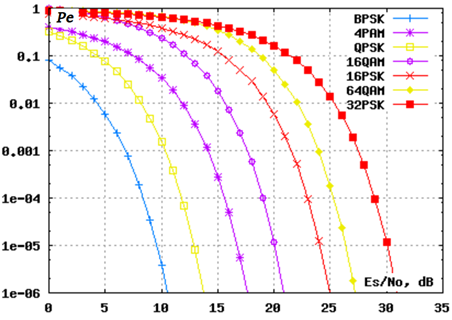
\includegraphics[scale=1]{Imagenes/Es.png}
	\label{fig:Es}
	%	\captionsetup{justification=raggedright,font={scriptsize,bf,it}}
	%	\caption*{fuente: \textcolor{
	%			Orange}{Tomada de Wikipedia}}
\end{figure}
%%%%%%%%%%%%%%%%%%%%%%%%%%%%%%%%%%%%%%%%%%%%%

\section{Técnicas de Corrección de Errores}

%%%%%%%%%%%%%%%%%%%%%%%%%%%%%%%%%%%%%%%%%%

\section{Técnicas de Duplexación}

%%%%%%%%%%%%%%%%%%%%%%%%%%%%%%%%%%%%%%%%%%%

\section{El multiplexado por Division de Frecuencias}

%%%%%%%%%%%%%%%%%%%%%%%%%%%%%%%%%%%%%%%%%%%

\section{El Multiplexado y el Multiacceso}
\subsection{Multi acceso por Division de Frecuencias}
\subsection{Multi acceso por Division de Tiempo}
\subsection{Multi acceso por Division de Códigos}

%%%%%%%%%%%%%%%%%%%%%%%%%%%%%%%%%%%%%%%%%%%
\section{Técnicas relacionadas con la Diversidad}
\subsection{Diversidad de Tiempo. Interleaving}
\subsection{Diversidad de Espacio. MIMO}
\subsection{Diversidad de Frecuencias. FH-SS}
\subsection{Diversidad de código. DS-SS}

%%%%%%%%%%%%%%%%%%%%%%%%%%%%%%%%%%%%%%%%%%%
\section{Técnicas de Corrección de Errores}